\documentclass[12pt]{article}

% The preamble here sets up a lot of new/revised commands and
% environments.  It's annoying, but please do *not* try to strip these
% out into a separate .sty file (which could lead to the loss of some
% information when we convert the file to other formats).  Instead, keep
% them in the preamble of your main LaTeX source file.
\usepackage[font=footnotesize]{caption}
\usepackage{float}
\usepackage{epsf}
\usepackage{epsfig}
\usepackage{subfigure}
% \usepackage{subfig}
\usepackage{latexsym}
%\usepackage{algorithm}
%\usepackage[noend]{algorithmic}
% \usepackage{color}
\usepackage{color, colortbl}
\usepackage{wrapfig}
\usepackage{topcapt}
\usepackage{multirow}
\usepackage{tabularx}
\usepackage{hyperref}
\usepackage{xcolor}
\usepackage{mdwlist}


%\usepackage{color}
\newcommand{\lc}[1]{\textcolor{blue}{#1}}


% \usepackage{amsmath, amsfonts, amssymb}
% \usepackage{algorithmic}
\usepackage[hmargin=1in,vmargin=1.2in]{geometry}
\usepackage{url}
\usepackage{multirow}
\usepackage[ruled,noline,linesnumbered]{algorithm2e}
\usepackage[bottom]{footmisc}
\usepackage{afterpage}
%\usepackage[caption=false]{caption}
\usepackage{eurosym}
\usepackage{enumitem}
% \usepackage{soul}
\usepackage{fancyhdr}
\usepackage{dashrule}
% \usepackage[stable]{footmisc}
% \usepackage{placeins}
% \setitemize{noitemsep,topsep=0pt,parsep=0pt,partopsep=0pt}
% \usepackage[utf8]{inputenc}
\usepackage{gensymb}
\usepackage{rotating}
\usepackage{tikz}


\widowpenalty=1000
\clubpenalty=1000

\def\rx{{\texttt{T-REX\ }}}
\def\rxe{{\texttt{T-REX}}}
\def\ls{{\texttt{LSTS\ }}}
\def\lse{{\texttt{LSTS}}}
\def\eut{{\texttt{EUROPA}$_2$\ }}
\def\eu{{\texttt{EUROPA}\ }}
\def\eue{{\texttt{EUROPA}}}
\def\eus{{\texttt{EUROPA}'s\ }}
\def\nd{{\texttt{NDDL\ }}}
\def\nde{{\texttt{NDDL}}}
\def\pd{{\texttt{PDDL\ }}}
\def\pde{{\texttt{PDDL}}}
\def\eur{{\texttt{EUROPtus\ }}}
\def\eure{{\texttt{EUROPtus}}}
\def\nas{{\texttt{NASA\ }}}
\def\nase{{\texttt{NASA}}}
\def\sml{{\texttt{SmallSat\ }}}
\def\smle{{\texttt{SmallSat}}}
\def\univ{{\texttt{UPorto\ }}}
\def\unive{{\texttt{UPorto}}}
\def\aut{{\texttt{Autonaut\ }}}
\def\aute{{\texttt{Autonaut}}}
\def\proj{{\textbf{PROTEAN\ }}}
\def\proje{{\textbf{PROTEAN}}}
\def\col{{\texttt{COLREGS\ }}}
\def\cole{{\texttt{COLREGS}}}

\def\etal{{et al.\/}}
\def\eg{e.g., }
\def\ie{{i.e.,\ }}
\def\etc{{etc.\ }}
\def\situ{{in situ \/}}
\def\PN{{\emph{PN} }}


\input{epsf}

%\usepackage{mathptmx}
%\usepackage{multirow}

\newcommand{\rtime}[1]{\par\noindent\rlap{#1} \hspace*{2.15cm}}
\newcommand{\iblank}{\par \noindent \hspace*{2.4cm} \hangindent 2.6cm}
\newcommand{\m}[1]{\ensuremath{\mathbf{#1}}}
\newcommand{\mc}[1]{\ensuremath{\mathcal{#1}}}
% \newcommand{\mb}[1]{\mbox{\boldmath$#1$\unboldmath}}
%\newcommand{\norm}[1]{\left| \left| #1 \right| \right| ^2}
\newcommand{\snr}{\hbox{SNR}}
\newcommand{\mse}{\hbox{MSE}}
\newcommand{\E}{{\mathbb E}}
\newcommand{\cn}{{\mathcal{CN}}}
\newcommand{\ba}{\begin{align*}}
\newcommand{\ea}{\end{align*}}

\newcommand{\real}{{\mathbb{R}}}
\newcommand{\integer}{{\mathbb{Z}}}
\renewcommand{\natural}{{\mathbb{N}}}
\newcommand{\argmin}{\operatorname{argmin}\displaylimits}
\newcommand{\argmax}{\operatorname{argmax}\displaylimits}

\newcommand{\relthresh}{{T_{\text{rel}}}}
\newcommand{\absthresh}{{T_{\text{abs}}}}

\newcommand{\nprof}{{N_{\text{prof}}}}
\newcommand{\DM}{{DM}}
\newcommand{\UM}{{UM}}
\newcommand{\deltaMax}{{\partial_{\max}}}
\newcommand{\IFD}{{IFD}}
\newcommand{\IFU}{{IFU}}

\newcommand{\mvdiff}{\mathbf{mvd}}
\newcommand{\mvest}{\widehat{\mvdiff}}
\newcommand{\prof}{p}

\newtheorem{Prop}{Proposition}
\newtheorem{Theorem}{Theorem}
\newtheorem{Lemma}{Lemma}
\newtheorem{Corrolary}{Corollary}

\def\be{\begin{equation}}
\def\ee{\end{equation}}

\newlength{\doublespacelength}
\setlength{\doublespacelength}{\baselineskip}
\addtolength{\doublespacelength}{0.5\baselineskip}
\newcommand{\doublespace}{\setlength{\baselineskip}{\doublespacelength}}

\newlength{\singlespacelength}
\setlength{\singlespacelength}{\baselineskip}
\newcommand{\singlespace}{\setlength{\baselineskip}{\singlespacelength}}


\newlength{\savedspacing}
\newcommand{\savespacing}{\setlength{\savedspacing}{\baselineskip}}
\newcommand{\restorespacing}{\setlength{\baselineskip}{\savedspacing}}

\setlength{\parskip}{0pt}
\setlength{\parsep}{0pt}
\setlength{\headsep}{0pt}
\setlength{\topskip}{0pt}
\setlength{\topmargin}{0pt}
\setlength{\topsep}{0pt}
\setlength{\partopsep}{0pt}
% \setlength{\parindent}{0pt}

\newcommand{\icomnt}[1]{{\color{red}{#1}}}
\newcommand{\kcomnt}[1]{{\color{blue}{#1}}}

\newcommand{\unit}[1]{\ensuremath{\mathrm{#1}}}                  %%%% to units and other roman math stuff
% \linespread{0.98}
% % \linespread{2.00}

\newcounter{quotenumber}

\newenvironment{numquote}{%
    \begin{enumerate}%
     \setcounter{enumi}{\value{quotenumber}}%
     \color{darkgray}
    \item \begin{quote}%
}{%
    \end{quote}%
    \setcounter{quotenumber}{\value{enumi}}
    \end{enumerate}%
}%

\makeatletter
\def\myitem{%
   \@ifnextchar[ \@myitem{\@noitemargtrue\@myitem[\@itemlabel]}}
\def\@myitem[#1]{\item[#1]\mbox{}}
\makeatother



\newcommand\blankpage{%
    \null
    \thispagestyle{empty}%
    \addtocounter{page}{-1}%
    \newpage}

\setcounter{secnumdepth}{0} 

\let\oldthebibliography\thebibliography
\let\endoldthebibliography\endthebibliography
\renewenvironment{thebibliography}[1]{
  \begin{oldthebibliography}{#1}
    \setlength{\itemsep}{0em}
    \setlength{\parskip}{0em}
}
{
  \end{oldthebibliography}
}
\linespread{0.98}
\parskip 0.1cm
\definecolor{Gray}{gray}{0.6}



%The next command sets up an environment for the abstract to your paper.

\newenvironment{sciabstract}{%
\begin{quote} \bf}
{\end{quote}}



% Include your paper's title here

\title{Towards a Robotic Ensemble for Ocean Observation} 


% Place the author information here.  Please hand-code the contact
% information and notecalls; do *not* use \footnote commands.  Let the
% author contact information appear immediately below the author names
% as shown.  We would also prefer that you don't change the type-size
% settings shown here.

\author
{John Smith,$^{1\ast}$ Jane Doe,$^{1}$ Joe Scientist$^{2}$\\
\\
\normalsize{$^{1}$Department of Chemistry, University of Wherever,}\\
\normalsize{An Unknown Address, Wherever, ST 00000, USA}\\
\normalsize{$^{2}$Another Unknown Address, Palookaville, ST 99999, USA}\\
\\
\normalsize{$^\ast$To whom correspondence should be addressed; E-mail:  jsmith@wherever.edu.}
}

% Include the date command, but leave its argument blank.

\date{}


\begin{document}

% ***********************************
% Uncomment the following for double space
% \baselineskip24pt
% ***********************************

\maketitle 

% Place your abstract within the special {sciabstract} environment.

\begin{sciabstract}
  The worlds oceans have been changing rapidly for some time; however
  the observational methods and capacity have hewed to the tradition
  of ship based approaches with discrete measurements to discern
  continuous processes in space and time.  The ongoing revolution in
  Robotics, Artificial Intelligence and sensor development are making
  rapid strides in how we are and likely to observe our global
  oceans. We believe it is only a matter of time for technology to
  make a sustained and large scale impact on how we observe the
  complexity of the upper ocean. The trajectory we take will however
  be important; we offer a perspective on an approach we believe will
  help solve the fundamental problem of undersampling with
  multi-domain ensembles of intelligent, networked robots.
  
  % JBS but this is just the beginning
  
  % It would be great to have a few diagrams depicting the structure
  % of the paper % Discussion of technological trends: # of vehicles will
  % increase significantly; new sats such as the ones from spaceX; from
  % vehicle systems to systems of systems; system-like or team-like
  % capabilities (find front; track front); immersive/viz holographic
  % realities; find correlations in data streams; % discussion of the
  % process for the paper: outline; get reactions; re-iterate
\end{sciabstract}

% \setcounter{secnumdepth}{2} 

\section{Introduction}

The world's oceans are a critical component for the habitability of
the 'pale blue dot' imaged by the Voyager mission (in 1990), that we
can call planet earth. Their photic zone with abundant phyto-plankton
produces the oxygen in every other breath we take. The ocean is a
living water mass with dynamic bio-geochemical processes that power
the abundance of plankton at the base of the human food chain.  Since
the industrial revolution, the oceans have absorbed increasing amounts
of anthropogenic CO\textsubscript{2} that humans have been spewing
into the atmosphere. They also provide a lifeline for the worlds
economies, a regulator of the planets weather and climate and also a
distinct source of relaxation and leisure activities. Yet the upper
ocean, arguably a small part of the worlds water-mass and our
interface to the ocean domain, is under-sampled and poorly understood
\cite{munk2002}. The principal problem in ocean science is to
understand the processes which power this part of the ocean and to do
so, we need to understand the ocean not just in space but also in
time, i.e. in 4D.

Traditional methods pioneered by Charles Darwin with his exploration
of new worlds on the \emph{Beagle}, have continued to drive how we
observe and sample the water-column as a means to understand
bio-geochemical processes typically with water-column measurements in
3D or 2D.  Modern research vessels typically make discrete water
sample measurements instrumented by lowering CTDs rosettes and
plankton nets which require the vessel to stop periodically. These
measurements are pulled together with assumptions about space/time
variability to discern what are continuous processes in space and
time. Underway measurements including those towed behind the research
vessel such as toyo's (\kc{cite}) provide continuous measurements but
are restricted to the vessels movement and have no independant means
to adapt to variability in the water-column. Eulerian and Lagrangian
approaches to observations such as buoys and \texttt{ARGO} floats
\cite{roemmich09} can make accurate assessments with temporal
variability and space and time respectively, but are constrained by
what water mass passes by. Driven by the Oil and Gas industry,
remotely operated vehicles (ROVs) are in a different class in of
themselves. As tethered vehicles, they've been immensely successful in
exploration where \emph{manipulation} rather than measurement is at
the core; this is particularly in the context of benthic exploration
including those involving marine science \cite{yoerger00,robi17} and
archeology \cite{coleman00}. ROVs however are not autonomous and not
the focus of this paper.


% As soon as you get to anything more sophisticated, the costs go up so
% much that the number of sensors is drastically reduced.  So we have to
% have a more "smart" way to sample and that is with platforms that can
% talk to each other and do intelligent sensing along the lines of what
% you are doing in your lab.  We need platforms that can follow isolines
% of variables of interest for example (or for that matter cut through
% isolines to find maxima in gradients).  And we need to ensure that
% these platforms are scalable - i.e. they can't be one of a kind, have
% to be designed as scalable (meaning inexpensive) from the beginning.
% My personal prejudice is that while it is wonderful that Woods Hole
% and MBARI are making those very fancy instruments, they alone are not
% going to change our understanding of the ocean.


Traditional methods in ocean science involved taking measurements
every few hundred miles to describe how we think the ocean works while
neglecting all higher frequencies of variability as noise.  As our
knowledge has progressed and we have learned over the last few decades
that the more we look, more important the smaller scale features are
and that they don't linearly scale to add to the large patterns we
used to describe the oceans. A great challenge therefore, has been to
understanding how oceans and the life in them work and how this is
changing, what the oceans might look like in the future, and this
challenge is one of sampling.  The current approach to increasing
sampling is to simply increase the number of samplers and thereby
increase the number of observations.

More recently, robotic vehicles have been augmenting traditional
ship-based observations, in the aerial, surface and underwater
domains. Simple buoyancy driven gliders, with hydrofoil wings and no
propulsion initiated this transition and have demonstrated sustained
in-water presence \cite{rucool11} as autonomous underwater vehicles
(AUVs). However, their adaptability to measure water-column properties
has been limited to straight line transects. Powered AUVs with
thrusters and larger electrically driven payloads have been making
inroads to this trend \cite{loch89,dorado2004,Bellingham07}. Equally,
with a larger onboard computational capacity, more sophisticated
control systems and algorithms have enabled these vehicles to adapt to
sensory signals from their scientific payload and demonstrate an
information gathering capability which is novel and likely to change
how water-column measurements are made
\cite{bellingham94,aosn93,ryan10,das11b,das15,fossum18,fossum18b}.

Autonomous surface vehicles (ASVs) have till recently directed more
towards security operations \cite{wolf10}. However recent innovations
in energy harvesting have resulted in a range of platforms driven by
waves \cite{waveglider,verfuss19} and wind \cite{gentemann20,ghani14},
have allowed for longer-duration presence on the oceans surface, often
a harsh environment.

While AUVs have become more acceptable in oceanographic observations,
it is interesting to note that both ASVs and unmanned aerial vehicles
(UAVs), have had a harder time gaining acceptance. The latter in
particular have been stymied by battery technology in being
circumscribed to operate near shore or via simple methods in launch
and recovery from a research vessel \cite{Ferreira2018}. Equally
payloads suitable both in mass and energy requirements for carrying on
such ship-launched platforms for over water observations have been
sparse compared to the rapid innovation in sensors for terrestrial
drones. This too however, is changing with low cost DMS sensors (to
measure outgassing of biological productivity) (\kc{cite}) and imagers
including hyper-spectral \cite{sigernes18} and infra-red sensors now
available for integration.

While substantial progress has been made in bringing each class of
these assets to aid and augment ocean observation, some more
effectively than others, less has been done to make effective use of
these vehicles in a sustainable and cohesive manner to actually make a
significant leap in ocean observation. To do so, we believe that in
adopting the following \textbf{four} ways, we can significantly
advance not just the science of ocean observation, but also a
systematically engineered approach to marine robotics.

First, the adoption of \emph{networked} robotics is critical to
increasing the sensing footprint of a research vessel. Making discrete
measurements of macro-phenomenon (e.g. blooms, anoxic zones, plumes of
any kind, fronts) across space and time, requires un-aliased sensing
which requires the presence of multiple sensory elements across a
large (typically on meso-scale $\sim 50$ Km\textsuperscript{2})
spatial extant. While eulerian or lagrangian sensors are possible,
practicality requirements in the open (or even coastal) ocean imply
the use of mobile robotic assets. For their placement and control,
networked methods to communicate and control are critical for
subsequent data assimilation and analysis.

Second, even if multiple robotic platforms (mobile or immobile) are
available and placed in an 'appropriate' location for making the
necessary measurements, if they do not \emph{adapt}, then a large
portion of the signal being tracked is likely to be missed or poorly
resolved, spatio-temporally (\kc{cite}).

Third, to look at phenomenon at scale, both high-resolution spatially
coherent data as also fine-scale temporal resolution is needed
(\kc{cite}) to separate bio-geophysical interactions, for instance in
wind-driven upwelling. \emph{Synoptic} views are therefore important
in resolving the scales of the processes in question, so both the
macro- perspective, provided by remote sensing and the micro view
provided by in-situ assets making continuous measurements are required
to be fused together.

Finally, a mix of predictive and reactive approaches are required to
be able to determine the central problem in oceanographic sampling,
i.e. ``where and when to sample''. And to do understand the
spatio-temporal aspects of this living mass in 4D to to zoom in and
out and map in and out large or smaller volumes and to look at micro
to macro structure. Ocean models driven by remote sensing and highly
non-linear computation can provide hindcasts, nowcasts and
forecasts. These can be valuable in event-response situations such as
oil spills and other forms of coastal marine pollution or natural
forcings that can cause blooms, for instance. However model skill in
making predictions with sufficient levels of confidence continues to
dodge coastal, sub-mesoscale and near-shore waters. Coupling models
with assimilated sensor measurements however, provide a way out to
increasing model skill and making predictions, especially in dynamic
mixed waters in the coastal environment.

To cover these approaches, we need an ensemble of robotic vehicles
with different sensors to be able to characterize different processes
at different scales and varying levels of synopticity. And to have
them coherently looking at one patch of the ocean over space, aerial,
surface and underwater domains and to be able to integrate
these measurements to provide a cogent ``MRI'' scan of the upper
water-column. And to do so, with as much automation in hardware and
platforms, as well as in software data synthesis, analysis and
decision making in an interdisciplinary manner merging ocean science,
robotics and Artificial Intelligence (AI) including Machine Learning
(ML). 


\begin{enumerate} 

%   \item Why do we observe the world's oceans? I.e. importance of the oceans
% themselves

% \item How do we observe?

\item What are its inherent limitations and why scientists do what
  they do; this to address the issues related to variability in the
  water-column, physics (e.g. type 1 vs type 2 regions), seasonal and
  temporal (e.g. tidal) variability. All packed as an oceanography 101
  type of material within a para or two

\item What is the focus of this m/s? Delineate upper water-column from the
meso-pelagic an down to the benthic.

\item A brief (1-2 sentence) history of ocean observation from Darwin to
Challenger and onwards, and the emphasis and need for ships.

\item talk about how ships themselves have evolved in some form
  (e.g. Falkor’s super-computer, and the viability of high-bandwidth
  comms to make remote work feasible (e.g. Bob Ballard’s Ocean Space
  Center and the R/V Nautilus)



\item Pulling apart biological from Phys., Chemical and Geological ocean
observation. 

\item How did Satellite remote sensing change the way ocean science has
been done and what impacts they've had

\end{enumerate}

\section{Robotics and AI in Ocean Observation}

\begin{wrapfigure}{!h}{2.7in}
  \centering
  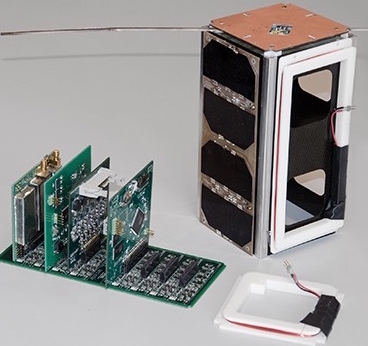
\includegraphics[width=0.4\textwidth]{fig/smallsat.png}
  \caption{\smle's are rapidly moving from technological curiosities
    to operational science platforms adept at earth observing remote
    sensing.}
  \label{fig:sats}
\end{wrapfigure}

The use of robotic assets in ocean observation is relatively
recent. While tethered and immobile 'robots' like moorings have
existed for some time to make in-situ measurements in place, mobile
robots starting with Lagrangian floats, followed by unpowered gliders
\cite{davis02} and now powered AUVs are increasingly making an impact
in scientific exploration. With the recent and ongoing revolution in
miniaturization of sensors, driven in large part by the Smartphone
technologies \cite{yang18}, the impact on marine robotics has been
particularly felt with increasing use of ASVs, many powered by wave or
wind action, and UAVs. ASV's in particular have been adopted widely
for maritime coastal defense \cite{huntsberger11} and monitoring
\cite{johnston17}. What is new is the use of UAVs, from shore and ship
for remotely sensed measurements including ocean color, DiMethyl
Sulfate (DMS), spotting megafauna or measuring the impact of pollution
\cite{dawson17,Ferreira2018,bayirhan19,wei19,pinto20}. Yet awaiting at
the margins of the robotic revolution is a platform, which could
vastly augment the range of applications and observations: the Small
Satellite, a low cost, often student built space vehicle which is
being encouraged as an educational artifact, yet has had little impact
to date on ocean observation \cite{guerra16}.

\smle's are a standardized platform, based on a 10 cm wide cube (1U)
with a mass of up to 1.3 kg with a aluminum based skeleton which can
be integrated with a range of commercial or bespoke instrumentation
(Fig. \ref{fig:sats}). The sizes and payloads can be scaled based on
platform requirements in multiples of this 1U design. The trend to
design and build smaller and more compact payloads, leveraging the
electronics revolution, permits such \smle's to deliver data in
comparable ways to legacy satellite platforms which often take years
to design, build, test and fly; \smle's can often be hoisted within a
year or two at significantly less cost. This has resulted in the use
of the latest hardware (and software) to perform remote sensing
operations hitherto only national or transnational agencies could do,
democratizing space technology. Another distinct advantage that they
offer is a significant reduction in revisit time to provide data over
a fixed region on earth which can often augment data from legacy space
systems. However, significant challenges remain in providing adequate
power, pointing accuracy and payload mass, all of which are part of
ongoing research efforts.

\begin{figure}[!t]
  \centering
  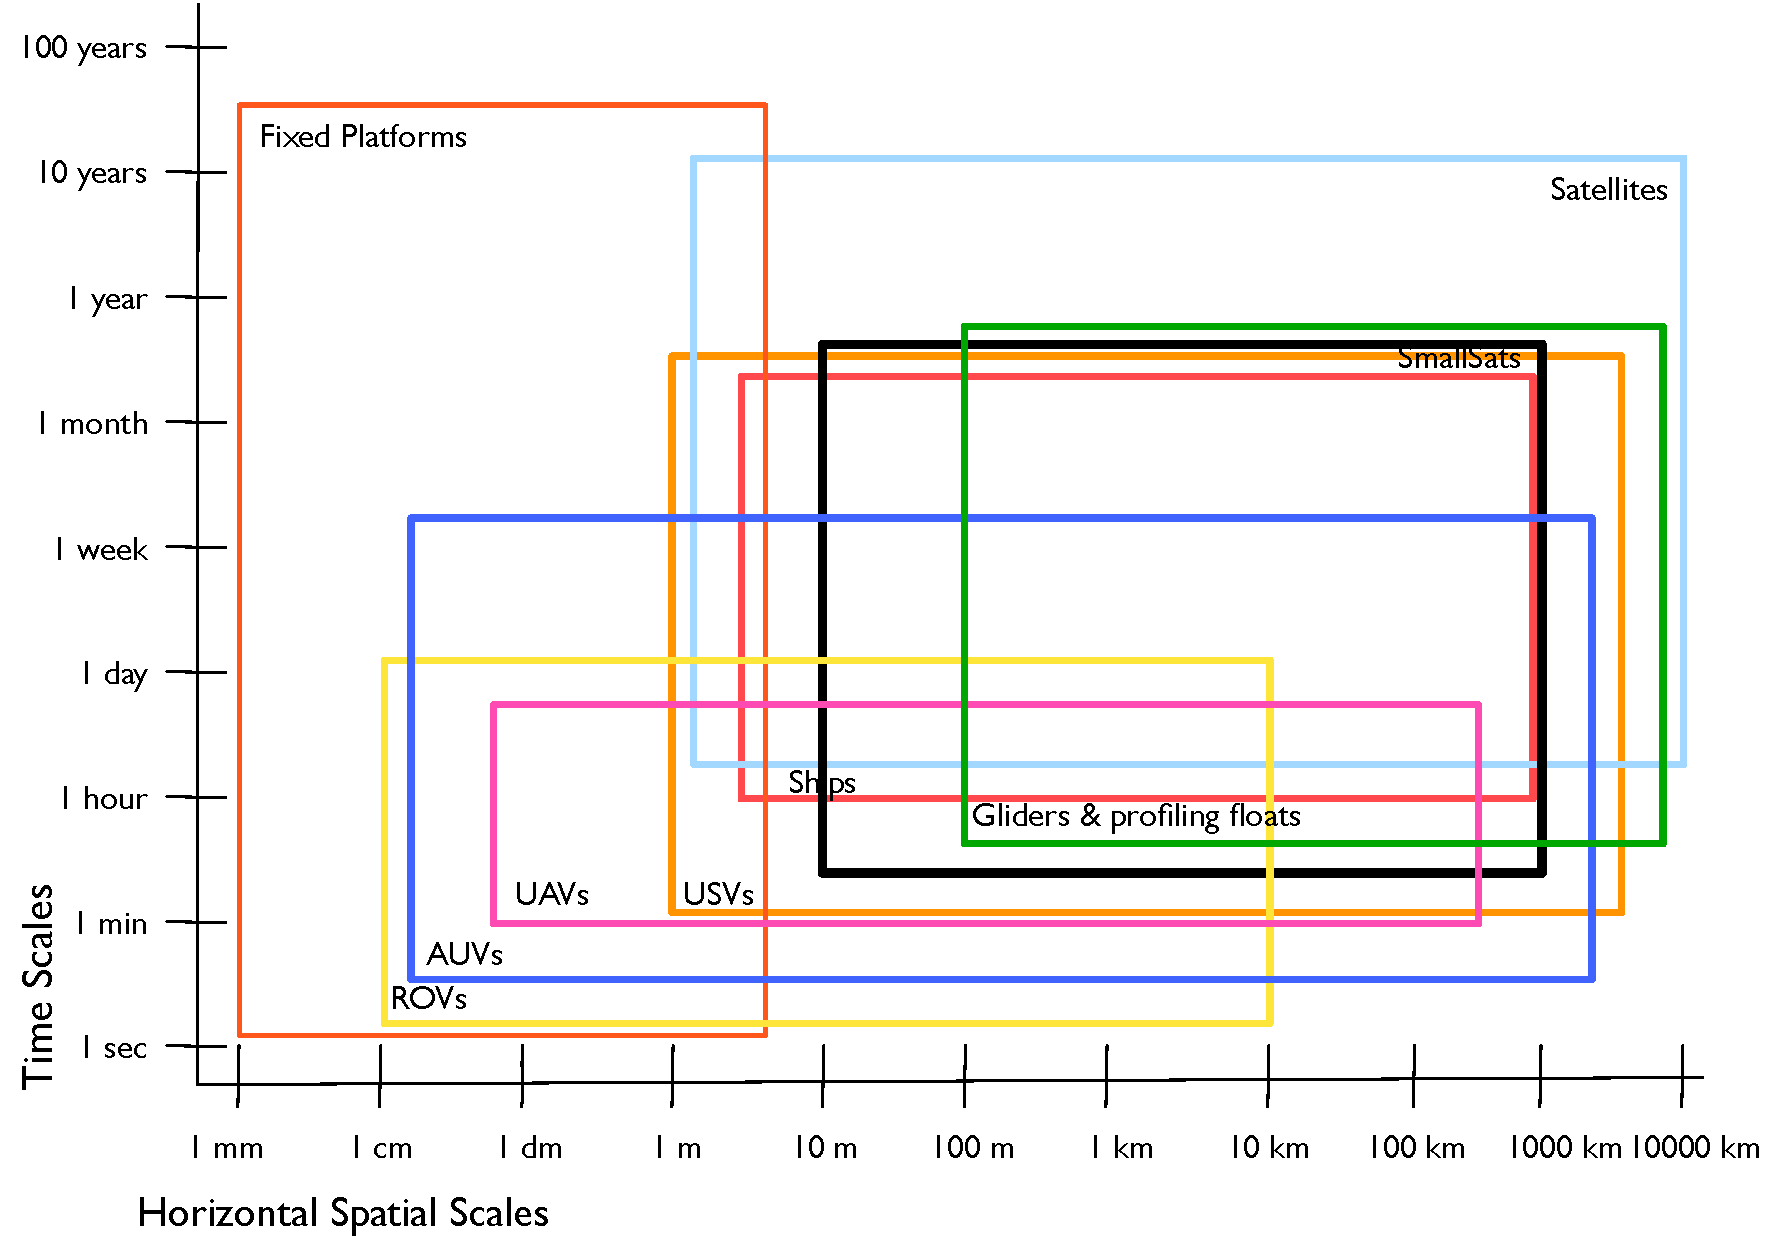
\includegraphics[width=0.7\textwidth]{fig/platform-capabilities.pdf}
  \caption{While \smle's do not occupy a unique position in ocean
    observation, overlapping a range of other assets, their capability
    for controlled observations along institutional lines is a
    harbringer of complementary views of the earths oceans. Figure
    modified from \cite{haury78}.}
  \label{fig:platforms}
\end{figure}

Fig. \ref{fig:platforms} shows how various robotic platforms' spatial
coverage maps into typical persistence in observation. Fixed platforms
such as moorings and buoys for instance, can be displaced a few meters
at most, but can provide observation continuity for decades if
maintained appropriately. Conversely platforms like UAVs can cover
vast distances, but their energy requirement constraints them to
operate at most a few hours. Powered AUVs with the latest battery
chemistry can operate up to a week while covering hundreds of
kilometers; gliders, can do better at slower speeds and cover larger
distances, yet their payload is constrained by onboard battery. 


\begin{wrapfigure}{!h}{2.7in}
  \centering
  \subfigure[]{\label{fig:platforms1}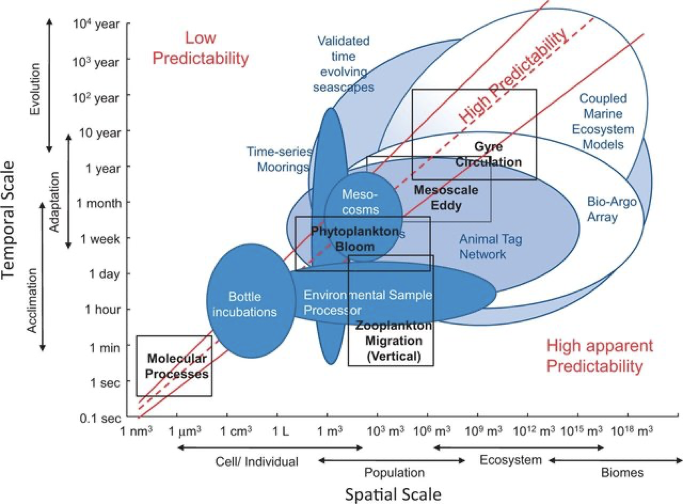
\includegraphics[width=0.5\textwidth]{fig/bio-processes.png}}
  \subfigure[]{\label{fig:platforms2}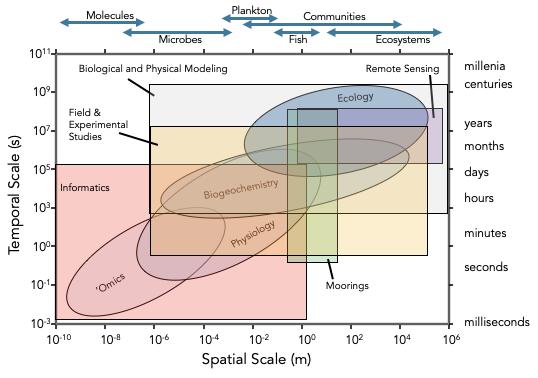
\includegraphics[width=0.5\textwidth]{fig/spatio-temporal.png}}
  \caption{\kc{Note these are placeholders from Ajit. I think these
      two figures can contribute to shaping the narrative quite a bit.}}
\end{wrapfigure}

While robotic platforms are critical to ocean observation, the
ultimate goal is to generate data from sensors which can be collated
and fused to provide \emph{information} in usable ways, to understand
causality, structure and process for the study of the upper
water-column. \kc{Need something meaty here to show what we mean by
  'fusing'} 

\subsection{AI and its application to Ocean Observation}

Much has been made of the revolution in data science and Machine
Learning (ML) in recent times, the impact of these sub-fields of
Artificial Intelligence and AI as a whole has been glancing. By 'AI'
we mean here the original notion of using logical formalisms tied to
computational decision making. At its heart lies the notion of
computational search where selection of possible outcomes of a
decision is informed either by a model, a heuristic or some principled
approach, so the outcome is deterministic if contextual. However the
conflating of data science and ML with 'AI' has added more confusion
than provided clarity in what researchers need to or ought to work on
to progress the science.

To understand causality of process function in the water-column, data
(e.g. temperature, salinity, oxygen, fluorescence, pH, \ldots) needs
to be collected and time-series need to be compiled over a period of
time to encompass tidal, seasonal and climatic variability. These are
typically adduced to generate some form of causal explanation for
human understanding that is at the heart of what is needed to create
knowledge about a changing planet. Where ML has provided insights in
the ocean sciences therefore has been on shore-side computation using
vast computing and data resources, post-facto to the actual
observational data collected \kc{Need citations}. A different effort
underway has been to use \emph{offline} neural network learned models
to actually impact \emph{online} observation making by a mobile robot
\cite{saad20} \kc{Add Yogi's mapping by surprise material
  here}. Separately, statistical methods in information theory, have
been used with far more practical outcomes to how a robot actually
samples in the water column
\cite{jdas13,das15,fossum18,fossum18b}. Newer methods in Statistical
ML applied to ocean sampling has also advanced the applicability in
where and when to sample in dynamic regions with discernable features
such as fronts and plumes \cite{fossum21}.

Where there has been markedly more effort and success, has been in the
\emph{control} of vehicles mostly on the surface or underwater, where
more systematic methods in AI have been brought to bear. Control of
such robots
\cite{benjamin2010,das11,das11b,olaya12,graham12,fossum18,fossum18b,pinto20}
including efforts for systematic coordination of aerial and underwater
vehicles \cite{Ferreira2018} as also some significant efforts in
mapping benthic communities \cite{johnson17} has been the hallmark of
efforts by technologists, to date.


% Lagrangian floats initiated the development of untethered
% devices, initially to measure sub-surface currents in the ocean via
% ocean acoustics. By being neutrally buoyant, these Lagrangian devices
% could then float with the current and periodically reach the surface,
% by changing their buoyancy, to communicate data and then return
% subsurface. Variations of float designs evolved into the design of an
% underwater glider with wings, a buoyancy engine and a method to shift
% weights to deal with pitch and yaw motion; this work was led by Doug
% Webb and Russ Davis \cite{davis02} motivated by a seminal article by
% Hank Stommel who imagined how glider fleets could traverse the worlds
% oceans over months making measurements while surveying vast stretches
% of the ocean \cite{stomme89}. While propelled vehicles were
% experimented upon as engineering artifacts \cite{blidberg01}, glider
% development for scientific exploration provided a filip to the use of
% AUVs.


% While research related to atmospheric phenomenon has long
% leveraged technology including remote sensing satellites, generating
% ocean measurements has been substantially more
% challenging. Observations from satellites cannot penetrate more than a
% few centimeters from the surface, sunlight does not permeate beyond
% the photic zone and crushing pressure requires instrumentation to be
% simple to operate yet robust to be able to survive. Terrestrial
% techniques in robot sensing and perception typically do not translate
% into making oceanographic measurements.

% The advent of lagrangian floats initiated the development of
% untethered devices, initially to measure sub-surface currents in the
% ocean via ocean acoustics. By being neutrally buoyant, these
% Lagrangian devices could then float with the current and periodically
% reach the surface, by changing their buoyancy, to communicate data and
% then return subsurface. Variations of float designs evolved into the
% design of an underwater glider with wings, a buoyancy engine and a
% method to shift weights to deal with pitch and yaw motion; this work
% was led by Doug Webb and Russ Davis \cite{davis02} motivated by a
% seminal article by Hank Stommel who imagined how glider fleets could
% traverse the worlds oceans over months making measurements while
% surveying vast stretches of the ocean \cite{stomme89}. While propelled
% vehicles were experimented upon as engineering artifacts
% \cite{blidberg01}, glider development for scientific exploration
% provided a filip to the use of AUVs.

While we are still at early stages of development of such platforms,
with sufficient computational and energy resources, yet their adoption
for science has proven to be surprisingly quick. Early adoption of
such 'robotic' vehicles from floats and gliders were traditionally
driven by the study of ocean physics (the study of currents,
acoustics, wind and the impact of bathymetry and surface
topology). More recent efforts however, have seeped into ocean biology
with the use of physical measurements as a means to understand the
presence and community structure of organisms from the micro to the
macro and highly inter-disciplinary studies of ecology of the coastal
as well as the deep ocean, thereby merging observations in physical
and bio-geochemical oceanography as a means to study ecosystems,
typically at the meso-scale. The emergence of ocean remote sensing has
also provided an inordinate amount of information about the upper
ocean, in ways that have previously been challenging to obtain,
especially at large spatio-temporal scales. Together, this has
resulted in the possibility of defining a new paradigm of ocean
observation and consequently of marine robotics. While the latter has
also had a profound impact from commercial Oil and Gas exploration
(especially with the advancement of tethered remotely operated
vehicles) and maritime defence, as also the use of \emph{immobile}
Eulerian 'robots' such as moored surface and sub-surface buoys, our
focus in this work is geared towards civilian oceanographic
observations using mobile platforms.


% Trace the advent of scientific instrumentation which morphed into
% floats, into gliders and powered AUVs.

% \begin{enumerate} 

%   % \item articulate the various 'robotic' vehicles, mobile and
%   %   immobile. Keep this general, so even a buoy is a robotic sensing
%   %   platform

%   \item how an ensemble of vehicles can extend the “reach" of the
%     human senses onboard the ship and perhaps even from shore with
%     high bandwidth comms -- extend the above to not just water-column,
%     but benthic work (where I know very little)

%   \item Show the figure of which robotic assets are viable for what
%     kinds of observation. Overlay bio-physical processes which are
%     appropriate and discuss at length why these assets suit those
%     specific observations.

%   \item Articulate how robots have 'extended the human senses' from
%     ship and shore to provide new ways of observing the ocean

%   \item In brief -- examples of Machine Learning and other forms of AI
%     which can help and how (see below). Machine Learning offline or
%     even inline in the perspective of “discovery"

%   \item How systematic observation, as against point measurements
%     (i.e. dipping a rosette) and using extrapolation, can help. What
%     kinds of signals are being missed

%   \item Harshness of the environment and operational issues of being
%     at sea for sustained presence

% \end{enumerate}

\section{Ocean models}

Articulate what models do, how they contribute and what their state of the art is. 
\section{On Sampling the water column}

\begin{enumerate} 

\item define sampling in the context of ocean science -- systematic
  measurement of variables over space and time, to be able to
  disambiguate cause-effect relationships

\item the importance of measuring variability in 4D (Space X
  Time). That vertical variability in the water-column is more
  pronounced 
  
\item why is it hard? Static-sensor/static field,
  static-sensor/dynamic field, mobile-sensor platform (AUVs
  etc)/dynamic field. Talk about aliasing of space/time. Refer to
  current methods from the Intro section.

\end{enumerate}

\section{New Horizons -- Bringing the two together -- Future trends in Ocean Science}

This could be the core of the m/s -- a look ahead to what we think the
contributions of AI and Robotics can do, leveraging networked vehicle
technologies, given large spatial extents to be sampled. 

\begin{enumerate} 

\item Implications of the use of robotic vehicles -- plusses and
  challenges. The role of vehicles in space, aerial, surface and
  underwater environments

\item how new generations of spacecraft (incl. SmallSats) could alter
  the landscape — e.g. our pitch to Audacious
  
\item How AI/ML can tie the needs of observational requirements and
  alleviate the issue of space/time and understanding spatio-temporal
  cause-effect relationships

\item The use of robots in security and surveillance. Legal implications
  related to use of robotic vehicles in such domains. 

\end{enumerate}

  
\section*{Concluding remarks}

% \begin{enumerate} 

% \end{enumerate}




\bibliography{references}

\bibliographystyle{Science}

\section*{Acknowledgments}

\section{Notes}

Notes from July 2nd conversation.

\begin{itemize}[noitemsep,topsep=0pt,parsep=0pt,partopsep=0pt]

\item The purpose of this work is to think of the ocean as a living
  water mass, with dynamic processes in the upper water-column.

\item This part of the water column and the photic zone and the
  productivity of this upper water column has a direct relationship with
  our existence on the planet by generating oxygen. Every other breath
  we take comes from phytoplankton generated oxygen.

\item The principal problem in ocean science is to understand the
  processes which power this part of the ocean. To do so, we need to
  understand the ocean not just in space but also in time, i.e. in
  4D. Typically we have been looking at water-column measurements in 3D
  or 2D.

\item We need to use such 4D visibility to zoom in and out, map in and
  out large or smaller areas.

\item And to augment process studies to enable looking from micro
  structure to the macro to understand the impact of the changing
  oceans.

\item Further, some processes might be visible to one and not the other
  sensor. Consequently, we will need to look at the ocean with multiple
  sensors at multiple resolutions, at varying levels of synopticity.

\item Therefore we need robotic platforms which can cover space and time
  in varying ways, and we need mechanisms to be able to integrate
  measurements across these different sensors and platforms.

\item And to do so, with as much automation as possible, to cover the
  vast stretches of often hostile and harsh oceans.

\item Data fusion and machine ``discovery'' will therefore be an
  important part of this narrative to enable panning thru troves of data
  once sensors and platforms are in place to observe.

\item Discovery will come in part from understanding the nature of
  ``surprise'' in data which is a part of exploration.

\item Understanding of Lagrangian Vs. Eularian methods of
  observation with constant environmental change. Example, observing a
  changing iceberg from below -- observe the change as the dynamics of
  the moving iceberg and its composition are constantly changing.

\item Using robots is not just about measuring at scale for space X
  time, and also not about measuring specific variables but in
  understanding the specific processes which we need to disambiguate.

\item Calibration of a range of sensors looking at the same patch of the
  ocean is a challenge.

\item Data fusion is another.

\item Need a figure which can be used to layer processes with
  sensors/platforms akin to the one from Scott Doney.

\end{itemize}

\newpage
\large{Be sure to see \url{https://www.sciencemag.org/node/2385628}
  for info on
  Sci. Robotics Perspectives and what they're looking for}\\


Potential folks to recruit, once we have a baseline draft:

\begin{enumerate}[noitemsep,topsep=0pt,parsep=0pt,partopsep=0pt]
\footnotesize{  
\item Jo Eidsvik (NO) NTNU, Trondheim -— Statistics and Sampling https://www.ntnu.edu/employees/jo.eidsvik
\item Rick Stumpf (US) NOAA — coastal oceanography -- https://www.gulfbase.org/people/dr-richard-p-stumpf
\item Catarina Magalhaes (PO) Univ. of Porto, CIIMAR — biological oceanography -- https://www2.ciimar.up.pt/team.php?id=85
\item Stef Williams (AUS) Univ. of Sydney — Marine Robotics -- https://www.sydney.edu.au/engineering/about/our-people/academic-staff/stefan-williams.html
\item Ralf Bachmeyer (DE) Univ. of Bremen, Germany — Marine Robotics -- https://www.marum.de/en/Prof.-Dr.-ralf-bachmayer.html
\item Yogi Girdhar (US), WHOI — Marine Robotics and ML -- https://www.whoi.edu/profile/ygirdhar/
\item Paulo Relvas (PO), Univ. of Algarve, Portugal — Phys. Oceanography -- https://www.ccmar.ualg.pt/users/prelvas
\item Marta Chantal Ribeiro (PO) Univ. of Porto, CIIMAR -— Maritime Law and MPA’s -— https://www2.ciimar.up.pt/team.php?id=279
\item Oliver Zelinskly (DE), Oldenberg, Germany -- Sensors and ML -- https://uol.de/en/icbm/marine-sensor-systems
\item Nadia Pinardo (IT) Bologna, Italy -- Phys. Oceanography -- https://www.unibo.it/sitoweb/nadia.pinardi/en
\item Oscar Scholfield (US) Rutgers -- biological oceanographer -- https://marine.rutgers.edu/team/oscar-schofield/  
\item Mark Moline (US) Univ. of Delaware -- biological oceanographer -- https://www.udel.edu/academics/colleges/ceoe/departments/smsp/faculty/mark-moline/
\item Pere Ridao (ES) Univ. of Girona -- Marine Robotics -- http://eia.udg.es/~pere/Pere\_Ridao\_Home\_Page/Short\_CV.html
\item Mandar Chitre (SG) National Univ. Singapore -- Marine Robotics
  and acoustics -- http://www.chitre.net/

}
\end{enumerate}


\end{document} 
